\documentclass[twoside,a4paper]{article}
\usepackage{geometry}
\geometry{margin=1.5cm, vmargin={0pt,1cm}}
\setlength{\topmargin}{-1cm}
\setlength{\paperheight}{29.7cm}
\setlength{\textheight}{25.3cm}

% useful packages.
\usepackage{amsfonts}
\usepackage{amsmath}
\usepackage{amssymb}
\usepackage{amsthm}
\usepackage{enumerate}
\usepackage{graphicx}
\usepackage{multicol}
\usepackage{fancyhdr}
\usepackage{layout}

% some common command
\newcommand{\dif}{\mathrm{d}}
\newcommand{\avg}[1]{\left\langle #1 \right\rangle}
\newcommand{\difFrac}[2]{\frac{\dif #1}{\dif #2}}
\newcommand{\pdfFrac}[2]{\frac{\partial #1}{\partial #2}}
\newcommand{\OFL}{\mathrm{OFL}}
\newcommand{\UFL}{\mathrm{UFL}}
\newcommand{\fl}{\mathrm{fl}}
\newcommand{\op}{\odot}
\newcommand{\Eabs}{E_{\mathrm{abs}}}
\newcommand{\Erel}{E_{\mathrm{rel}}}

\begin{document}

\pagestyle{fancy}
\fancyhead{}
\lhead{NAME Jiatu Yan}
\chead{Numerical Analysis homework \#4}
\rhead{Date}


\section*{I. \small{Determine $p\in\mathbb{P}_3$ such that $s\left( 0 \right)=0 $.}}

We know $p\left( 0 \right)=0 $, $p\left( 1 \right)=s\left( 1 \right) =1 $
, $p'\left( 1 \right) =s'\left( 1 \right)=3 $
, $p''\left( 1 \right) =s''\left( 1 \right)=6 $
, thus we have:

\begin{tabular}{c|cccc}
x\\
0 &0\\
1 &1  &1\\
1 &1  &3  &2\\
1 &1  &3  &3 &1\\
\end{tabular}

So we have
\[
	p\left( x \right)=x+2x\left( x-1 \right)+x\left( x-1 \right)^2=x^{3}   
.\] 

Because $s\left(  0\right)=0^{3}=0 $, $s\left( 2 \right)=\left( 2-2 \right)^{3}=0  $, $s\left( x \right) $ is a natural cubic spline.

\section*{II. \small{Consider interpolation $f$ on  $[a,b]$ with a quadratic spline  $s\in\mathbb{S}^{1}_2$.}}

\subsection*{II-a \small{Why an additional condition is needed to determine s uniquely?.}}

$s\left( x \right) $ is constructed by $n-1$ polynomials with degree of 2, we can assume them $\{p_i\}$
, $s\left( x \right)=p_i\left( x \right)  $ when $x\in[x_{i},x_{i+1}]$.
Suppose $p_i=a_{i_2} x^2+a_{i_1} x+a_{i_0}$ so we have $3n-3$ variables. 

By the property of $s\left( x \right) $, we have $p_i\left( x_i \right)=f_i$ 
, $p_i\left( x_{i+1} \right)=f_{i+1}$
and $p_i'\left( x_{i+1} \right)=p_{i+1}'\left( x_{i+1} \right) $.
In the formal two equations $i=1,2\ldots,n-1$, while in the last one $i=1,2\ldots,n-2$. 
They construct $\left( n-1 \right)+\left( n-1 \right)+\left( n-2 \right)=3n-4$ equations.

The number of equations is less than that of variables, so we cannot determine s uniquely unless we introduce an additional condition.

\subsection*{II-b \small{Determine $p_i$ in terms of  $f_i,f_{i+1},$ and $m_i$ for  $i=1,2\ldots,n-1$}}

For $i=1,2\ldots,n-1$, we have $p_i\left( x_i \right)=f_i$, $p_i\left( x_{i+1} \right)=f_{i+1} $, $p_{i}'\left( x_{i} \right)=m_{i} $.
So

\begin{tabular}{c|ccc}
x\\
$x_i$     &$f_i$\\
$x_i$     &$f_i$  &$m_i$\\
$x_{i+1}$ &$f_{i+1}$  &$\frac{f_{i+1}-f_i}{x_{i+1}-x_i}$  
	  &$\frac{f_{i+1}-f_i-\left( x_{i+1}-x_i \right)m_i }{\left( x_{i+1}-x_i \right)^2 }$\\
\end{tabular}

Thus we have 
$$p_i\left( x \right)=f_i+m_i\left( x-x_i \right)
+ \frac{f_{i+1}-f_i-\left( x_{i+1}-x_i \right)m_i }{\left( x_{i+1}-x_i \right)^2}\left( x-x_i \right)^2  .$$

\subsection*{II-c \small{Suppose $m_1=f'\left( a \right) $ is given. Show how $m_2,\ldots,m_{n-1}$ can be compouted.}}

Because $p_i'\left( x_{i+1}\right)=p_{i+1}'\left( x_{i+1} \right)=m_{i+1} \quad i=1,2\ldots,n-2 $.
Since we have got the form of $p_i$. 
So we can calculate the derivative of  $p_i$ on  $x_{i+1}$,
\[
	p_i'\left( x_{i+1} \right)=m_i+2\frac{f_{i+1}-f_i-\left( x_{i+1}-x_i \right)m_i }{x_{i+1}-x_i} 
.\] 
Put it into the formal equation we have
\[
	m_{i+1} =\frac{2\left( x_{i+1}-f_i \right) }{x_{i+1}-x_i}-m_i \quad i=1,2,\ldots,n-1
.\] 
As we have known $m_1$, we can get all  $m_i$ by iteration.

\section*{III \small{Determine $s_2\left( x \right)$ on $[0,1]$. }}

Since s is a natural cubic spline, we have $s''\left(  -1\right)=s''\left( 1 \right)=0 $ 
, $s_2\left(  0\right)=s_1\left( 0 \right)=1+c  $
, $s_2'\left( 0 \right)=s_1'\left( 0 \right)=3c$, $s_2''\left( 0 \right)=s_1''\left( 0 \right)=6c  $.  

Now we suppose $x_1=-1,x_2=0,x_3=1$, $M_i=s''\left( x_i \right) \quad \left( i=1,2,3 \right) $.
So $M_2=6c$,$M_1=M_3=0$. Thus we have
\[
	s_2'''\left( 0 \right)=\frac{M_3-M_2}{x_3-x_2}=-6c 
.\] 
By using the Taylor expansion of $s_2\left( x \right) $ on $x_2$ we have
\[
	s_2\left( x \right)=s\left( 0 \right)+s'\left( 0 \right)x+\frac{M_2}{2}x^2+\frac{s'''\left( 0 \right) }{6}x^{3}
	=-cx^{3}+3cx^2+3cx+c+1
.\]
If we want $s\left( 1 \right)=-1 $, then we get $c=-\frac{1}{3}$. 

\section*{IV \small{Consider $f\left( x \right)=\cos\left( \frac{\pi}{2}x \right)$ with $x\in[-1,1]$}}

\subsection*{IV-a \small{Determine the natural cubic spline interpolant to f on knots -1,0,1.}}

We suppose that $x_1=-1,x_2=0,x_3=1$, $M_i=s''\left( x_i \right)$.
We have $s\left( x_1 \right)=f\left( x_1 \right)=0$,$s\left( x_2 \right)=f\left( x_2 \right)=1  $ 
, $s(\left( x_3 \right)=f\left( x_3 \right)=0 $.

The divided differences of f are

\begin{tabular}{c|ccc}
x\\
-1 &0\\
0  &1  &1\\
1  &0  &-1  &-1\\
\end{tabular}

So we can calculate $M_2$ by the equation $\mu_2 M_1+2M_2+\lambda_2M_3=f[x_1,x_2,x_3]$
, where $\mu_2=\frac{x_2-x_1}{x_3-x_1}$, $\lambda_2=\frac{x_3-x_2}{x_3-x_1}$.
We have $M_2=-3$. 

Since $s_i'\left( xi \right)=f[x_i,x_{i+1}]-\frac{1}{6}\left( M_{i+1}+2M_i\right)\left( x_{i+1}-x_i \right)  $,
we get $s\left( x \right) $ by using the Taylor expansion of $s\left( x \right) $ at $x_i$.

 \[
	 s_1\left( x \right)=\left( 1-\frac{1}{6}\left( -3 \right)  \right)\left( x+1 \right)+\frac{-3}{6}\left( x+1 \right)^{3}  
	 =-\frac{1}{2}x^{3}-\frac{3}{2}x^2+1
 .\] 
 \[
	 s_2\left( x \right)=1+\left( -1-\frac{1}{6}\left( -6 \right)  \right)x-\frac{3}{2}x^2+\frac{3}{6}x^{3}
	 =\frac{1}{2}x^{3}-\frac{3}{2}x^2+1
 .\] 

 \subsection*{IV-b \small{Verify the minimal total bending energy by taking $g\left( x \right) $}}

 The divided differences of f are

\begin{tabular}{c|ccc}
x\\
-1 &0\\
0  &1  &1\\
1  &0  &-1  &-1\\
\end{tabular}

So by Newton's formula we have 
\[
g\left( x \right)=\left( x-x_1 \right)-\left( x-x_1 \right)\left( x-x_2 \right)=-x^2+1  
.\] 
So $g''\left( x \right)=-2 $
\[
	\int_{-1}^{1}[s''\left( x \right)]^2dx=\int_{-1}^{0}\left( -3x-3 \right)^2dx+\int_{0}^{1}\left( 3x-3 \right)^2dx
	=6
.\] 
\[
	\int_{-1}^{1}[g''\left( x \right) ]^2dx=\int_{-1}^{1}4dx=8>6 
.\] 
Because $f''\left( x \right)=-\frac{\pi^2}{4}\cos\left( \frac{\pi}{2}x \right)  $, we have
\[
	\int_{-1}^{1}[f''\left( x \right)]^2dx=\frac{\pi^{4}}{16}\int_{-1}^{1}\frac{\cos\left( \pi x \right)-1 }{2}dx 
=\frac{\pi^{4}}{16}>6
.\] 
So we have $\int_{-1}^{1}[s''\left( x \right)]^2dx>\int_{-1}^{1}[g''\left( x \right)]^2dx  $
and $\int_{-1}^{1}[s''\left( x \right)]^2dx>\int_{-1}^{1}[f''\left( x \right)]^2dx $.

\section*{V \small{The quadratic B-splines $B^{2}_i\left( x \right) $.}}

\subsection*{V-a \small{Derive the same explicit expression of $B^{2}_i\left( x \right) $}}

We already have 
\[ B^{0}_{i}\left( x \right)=\left\{
	\begin{aligned}
		&1\qquad x\in (t_{i-1},t_{i}]\\
		&0\qquad otherwise\\
	\end{aligned}
	\right.
\] 
So by 
\[
	B^{1}_{x}=\frac{x-t_{i-1}}{t_i-t_{i-1}}B^{0}_{i}\left(  x\right)+\frac{t_{i+1}-x}{t_{i+1}-t_i}B^{0}_{i+1}\left( x \right)  
.\] 
We have 
\[
B^{1}_{i}\left( x \right)=\left\{
	\begin{aligned}
		&\frac{x-t_{i-1}}{t_{i}-t_{i-1}}&\qquad x\in(t_{i-1},t_i]\\
		&\frac{t_{i+1}-x}{t_{i+1}-t_i}&\qquad x\in(t_i,t_{i+1}]\\
		&0&\qquad otherwise\\
	\end{aligned}
\right.\]
Since $B^{2}_{i}\left( x \right)=\frac{x-t_{i-1}}{t_{i+1}-t_{i-1}}B^{1}_{i}\left( x \right)
+\frac{t_{i+2}-x}{t_{i+2}-t_{i}}B^{1}_{i+1}\left( x \right)   $ 
When $x\in(t_{i-1},ti]$, $B^{1}_{i+1}=0$, we have
\[
	B^{2}_{i}\left( x \right)= \frac{x-t_{i-1}}{t_{i+1}-t_{i-1}}\frac{x-t_{i-1}}{t_{i}-t_{i-1}}
.\] 
When $x\in(t_{i+1},t_{i+2}]$, $B^{1}_{i}=0$, we have
\[
	B^{2}_{i}\left( x \right)=\frac{t_{i+2}-x}{t_{i+2}-t_{i}}\frac{t_{i+2}-x}{t_{i+2}-t_{i+1}} 
.\]
When $x\in(t_i,t_{i+1}]$, we have
\[
	B^{2}_{i}\left( x \right)=\frac{x-t_{i-1}}{t_{i+1}-t_{i-1}}\frac{t_{i+1}-x}{t_{i+1}-t_i}
	+\frac{t_{i+2}-x}{t_{i+2}-t_{i}}\frac{x-t_{i}}{t_{i+1}-t_{i}}
.\] 
So 
\[
	B^{2}_{i}\left( x \right)=\left\{
		\begin{aligned}
			&\frac{x-t_{i-1}}{t_{i+1}-t_{i-1}}\frac{x-t_{i-1}}{t_{i}-t_{i-1}}&\quad x\in(t_{i-1},t_{i}]\\
			&\frac{x-t_{i-1}}{t_{i+1}-t_{i-1}}\frac{t_{i+1}-x}{t_{i+1}-t_i}
			+\frac{t_{i+2}-x}{t_{i+2}-t_{i}}\frac{x-t_{i}}{t_{i+1}-t_{i}}&\quad x\in(t_i,t_{i+1}]\\
			&\frac{t_{i+2}-x}{t_{i+2}-t_{i}}\frac{t_{i+2}-x}{t_{i+2}-t_{i+1}}&\quad x\in(t_{i+1},t_{i+2}]\\ 
		\end{aligned}
\right.\] 

\subsection*{V-b \small{Verify that $\frac{d}{dx}B^{2}_{i}\left( x \right) $ is continuous at $t_i$ and $t_{i+1}$.}}

Since $B^{2}_{i}\left( x \right)$ are polynomials of degree 2
, it is obvious that $\frac{d}{dx}B^{2}_{i}\left( x \right) $ is continuous on $\left(  t_{i-1},t_{i+2}\right) $ 
except $t_{i}$ and $t_{i+1}$.

When $x=t_{i}$, we have
\begin{equation*}
	\begin{split}
	\lim_{x\to t_i^{+}}\frac{d}{dx}B^{2}_{i}\left( x \right) 
	&=\lim_{x\to t_i^{+}}\frac{2\left( x-t_{i-1} \right) }{\left( t_{i+1}-t_{i-1} \right)\left( t_{i}-t_{i-1} \right)  }
	=\frac{2}{t_{i+1}-t_{i-1}}\\
	\lim_{x\to t_i^{-}}\frac{d}{dx}B^{2}_{i}\left( x \right) 
	&=\lim_{x\to t_i^{-}}\frac{t_{i+1}+t_{i-1}-2x}{\left( t_{i+1}-t_{i-1} \right)\left( t_{i+1}-t_{i} \right)  }
	+\frac{t_{i+2}+t_{i}-2x}{\left( t_{i+2}-t_{i} \right)\left( t_{i+1}-t_{i} \right)  }\\
	&=\frac{t_{i+1}+t_{i-1}-2t_i}{\left( t_{i+1}-t_{i-1} \right)\left( t_{i+1}-t_{i} \right) }
	+\frac{t_{i+2}+t_{i}-2t_i}{\left( t_{i+2}-t_{i} \right)\left( t_{i+1}-t_{i} \right)  }
	=\frac{2}{t_{i+1}-t_{i-1}}
.
\end{split}
\end{equation*}

Because $\lim_{x\to t_i^{+}}\frac{d}{dx}B^{2}_{i}\left( x \right)=\lim_{x\to t_i^{-}}\frac{d}{dx}B^{2}_{i}\left( x \right) $
, we have $\frac{d}{dx}B^{2}_{i}$ is continuous on $t_{i}$.

Similiarly we can prove that
$\lim_{x\to t_{i+1}^{+}}\frac{d}{dx}B^{2}_{i}\left( x \right)=\lim_{x\to t_{i+1}^{-}}\frac{d}{dx}B^{2}_{i}\left( x \right) 
=\frac{-2}{t_{i+2}-t_{i}}$
, which means $\frac{d}{dx}B^{2}_{i}$ is also continuous on $t_{i+1}$.

\subsection*{V-c \small{Show that only one $x^{*}\in\left( t_{i-1},t_{i+1} \right) $ satisfies 
$\frac{d}{dx}B^{2}_{i}\left(  x^{*}\right)=0 $.}}
When $x\in(t_{i-1},t_{i})$, $\frac{d}{dx}Bi^{2}_{i}\left( x \right)=\frac{2\left( x-t_{i-1} \right) }{t_{i+1}-t_{i-1}}>0 $ 

When $x\in\left( t_{i+1},t_{i+2} \right) $ 
, $\frac{d}{dx}B^{2}_{i}\left( x \right)=\frac{2\left( x-t_{i+2} \right) }{t_{i+2}-t_{i+1}}<0 $ 

Since $\frac{d}{dx}B^{2}_{i}\left( x \right) $ is continuous on $\left( t_{i-1}, t_{i+2} \right) $ 
and is a polynomial with degree 1
, there exists only one $x^{*}\in\left( x_{i},x_{i+1} \right) $ satisfies that $\frac{d}{dx}B^{2}_{i}\left( x^{*} \right)=0 $.

So we have
\begin{equation*}
	\begin{split}
		\frac{d}{dx}B^{2}_{i}\left( x^{*} \right)
		=\frac{t_{i+1}+t_{i-1}-2x^{*}}{\left( t_{i+1}-t_{i-1}\right)\left( t_{i+1}-t_{i} \right)  }
		+\frac{t_{i+2}+t_{i}-2x^{*}}{\left( t_{i+2}-t_{i} \right)\left( t_{i+2}-t_{i} \right)  }=0&\\
		\Longrightarrow\left( t_{i+1}+t_{i-1}\right)\left( t_{i+2}-t_{i} \right)+\left( t_{i+2}+t_{i} \right)\left( t_{i+1}-t_{i-1} \right)
		-2x^{*}\left( t_{i+2}-t_{i}+t_{i+1}-t_{i-1} \right)=0&\\
		\Longrightarrow x^{*}=\frac{t_{i+1}t_{i+2}-t_{i-1}t_{i}}{t_{i+1}-t_{i-1}+t_{i+2}-t_{i}}.&
	\end{split}
\end{equation*}

\subsection*{V-d \small{Consequently, show $B^{2}_{i}\left( x \right)\in[0,1) $.}}

Because $\lim_{x\to t_{i-1}}B^{2}_{i}\left( x \right)=B^{2}_{i}\left( t_{i+2} \right)=0  $ 
,$B^{2}_{i}\left( x \right) >0$ when $x\in\left( t_{i-1} ,x^{*}\right) $ and  $B^{2}_{i}\left( x \right) <0$ when $x\in\left(x^{*},t_{i+2}\right)$. We can easily get $B^{2}_{i}\left( x \right)\ge 0 $.

By the property of $\frac{d}{dx}B^{2}_{i}\left( x \right) $, we can know that $B^{2}_{i}\left( x \right) $ will reach its maximum
at $x^{*}$. Then we have
\begin{equation*}
	\begin{split}
		\frac{d}{dx}B^{2}_{i}\left( x^{*} \right)
		&=\frac{\left( t_{i+1}-t_{i-1}\right)\left( t_{i+2}-t_{i-1} \right)\left( t_{i+1}-t_{i} \right)\left( t_{i+1}-t_{i-1} \right)}
		{\left( t_{i+1}-t_{i-1}+t_{i+2}-t_{i} \right)^2\left( t_{i+1}-t_{i} \right)\left( t_{i+1}-t_{i-1} \right)   } +
		\frac{\left( t_{i+2}-t_{i-1} \right)\left( t_{i+2}-t_{i} \right)\left( t_{i+2}-t_{i} \right)\left( t_{i+2}-t_{i} \right)    }
		{\left( t_{i+2}-t_{i-1}+t_{i+2}-t_{i} \right)^2\left( t_{i+2}-t_{i} \right)\left( t_{i+1}-t_{i} \right)   }\\
		&=\frac{t_{i+2}-t_{i-1}}{t_{i+2}-t_{i-1}+t_{i+1}-t_{i}}
	\end{split}
\end{equation*}
Since $t_{i+2}-t_{i-1}>0$ and $t_{i+1}-t_{i}>0$, we have $B^{2}_{i}\left( x^{*} \right)<1 $.
So $B^{2}_{i}\left( x \right) \in[0,1)$.

\subsection*{V-e \small{Plot $B_{i}^{2}\left( x \right) $ for $t_{i}=i$.}}

\begin{center}
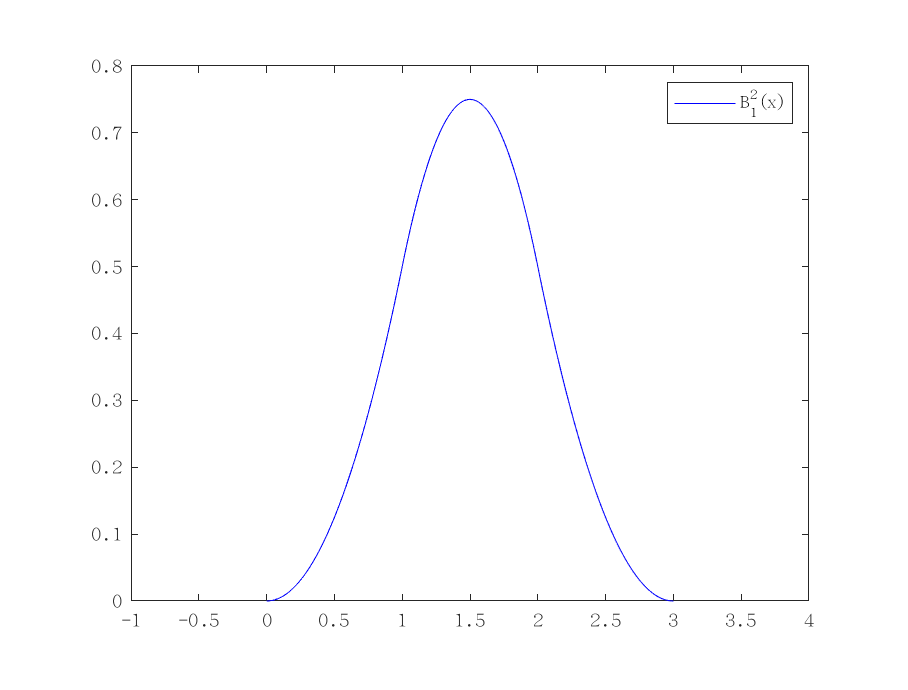
\includegraphics[width=10cm, height=5cm]{Plot.eps}
\end{center}

\section*{VI \small{Verify $\left( t_{i+2}-t_{i-1} \right)[t_{i-1},t_{i},t_{i+1},t_{i+2}]\left( t-x \right)_{+}^{2}  $ algebraically.}}

Because
$$ B^{0}_{i}\left( x \right)=\left\{
        \begin{aligned}
		&1\qquad x∈(t_{i-1},t_{i}]\\
                &0\qquad otherwise\\
        \end{aligned}
\right.$$
\begin{equation*}
	\begin{split}
		\left( t_{i}-t_{i-1} \right)[t_{i-1},t_{i}]\left( t-x \right)_{+}^{0}
		&=\left( x-t_{i-1} \right)_{+}^{0}-\left( x-t_{i} \right)_{+}^{0}\\
		&=\left\{
			\begin{aligned}
				&1\qquad x\in (t_{i-1},t_{i}]\\
				&0\qquad otherwise\\
			\end{aligned}
		\right.
	\end{split}
\end{equation*}
We can easily have $B_{i}^{0}\left( x \right)=\left( t_{i}-t_{i-1} \right)[t_{i-1},t_{i}]\left( t-x \right)^{0}_{+}$

Before proving the equation, we firsly calculate the ddivided difference of (t-x)

\begin{tabular}{c|cccc}
t\\
$t_{i-1}$&$\left( t_{i-1}-x \right)$ & \\
$t_{i}$  &$\left( t_{i}-x \right) $  &1&\\
$t_{i+1}$&$\left( t_{i+1}-x \right)$ &1&0&\\
$t_{i+2}$&$\left( t_{i+2}-x \right)$ &1&0&0\\
\end{tabular}

So from $\left( t-x \right)_{+}^{1}=\left( t-x \right)\left( t-x \right)_{+}^{0}$ and 
$\left( t-x \right)_{+}^{2}=\left(t-x  \right)\left( t-x \right)_{+}^{1}  $ we have

\begin{equation*}
	\begin{split}
		\left( t_{i+1}-t_{i-1} \right)[t_{i-1},t_{i},t_{i+1}] \left( t-x \right)_{+}^{1}
		&=\left( t_{i+1}-t_{i-1} \right)[t_{i-1}]\left( t-x \right)[t_{i-1},t_{i},t_{i+1}] \left( t-x \right)_{+}^{0}\\
	      &\quad+\left( t_{i+1}-t_{i-1}\right) [t_{i-1},t_{i}]\left( t-x \right) [t_{i},t_{i+1}]\left( t-x \right)_{+}^{0}\\
		&=\left( t_{i-1}-x \right)[t_{i},t_{i+1}]\left( t-x \right)_{+}^{0}-\left( t_{i-1}-x \right)[t_{i-1},t_{i}]\left( t-x \right)_{+}^{0}\\
		&\quad+\left( t_{i+1}-t_{i-1} \right)[t_{i},t_{i+1}]\left( t-x \right)_{+}^{0}\\
		&=\frac{x-t_{i-1}}{t_{i}-t_{i-1}}B_{i}^{0}\left( x \right)+\frac{t_{i+1}-x}{t_{i+1}-t_{i}}B_{i}^{0}\left( x \right)\\
		&=B_{i}^{1}\left( x \right).\\
		\left( t_{i+2}-t_{i-1} \right)[t_{i-1},t_{i},t_{i+1},t_{i+2}]\left( t-x \right)_{+}^{2}
		&=\left( t_{i+2}-t_{i-1} \right)[t_{i-1}]\left( t-x \right)[t_{i-1},t_{i},t_{i+1},t_{i+2}]\left( t-x \right)_{+}^{1}\\
		&\quad+\left( t_{i+2}-t_{i-1} \right)[t_{i-1},t_{i}]\left( t-x \right)
		[t_{i},t_{i+1},t_{i+2}]\left( t-x \right)_{+}^{1}\\
		&=\left( t_{i-1}-x \right)\left( [t_{i},t_{i+1},t_{i+2}]\left( t-x \right)_{+}^{1}-[t_{i-1},t_{i},t_{i+2}]\left( t-x \right)_{+}^{1}   \right)\\
		&\quad+\left( t_{i+2}-t_{i-1} \right)[t_{i},t_{i+1},t_{i+2}]\left( t-x \right)_{+}^{1}\\
		&=\frac{x-t_{i-1}}{t_{i+1}-t_{i-1}}B_{i}^{1}\left( x \right)
		+\frac{t_{i+2}-x}{t_{i+2}-t_{i}}B_{i}^{1}\left( x \right)\\
		&=B_{i}^{2}\left( x \right)\\ 
\end{split}
\end{equation*}

So we have proved that $B_{i}^{2}\left( x \right)=\left( t_{i+2}-t_{i-1} \right)[t_{i-1},t_{i},t_{i+1},t_{i+2}]\left( t-x \right)_{+}^{2}$.
\end{document}

%%% Local Variables: 
%%% mode: latex

%%% End: 
